\PassOptionsToPackage{english,ngerman}{babel}

\documentclass[a4paper,11pt]{article}

\usepackage{../style/thga-db}
\usetikzlibrary{positioning,calc}

% ============================================================
% Document metadata
% ============================================================

\renewcommand{\thgaKurs}{Developer Manual -- Filament Manager}
\renewcommand{\thgaDozent}{Stephan Bökelmann}
\renewcommand{\thgaEmail}{sboekelmann@ep1.rub.de}
\renewcommand{\thgaDatum}{\today}

% ------------------------------------------------------------
% Custom header and footer for the Developer Manual
% ------------------------------------------------------------

\fancyhead[L]{%
  \small\textcolor{THGABlau}{%
    \textbf{Developer Manual -- Filament Manager}%
  }%
}

\fancyhead[R]{%
  \small\textcolor{THGAGrau}{%
    Daniel Brendebach \ · \ \thgaDatum%
  }%
}

\fancyfoot[L]{}
\fancyfoot[C]{%
  \small\textcolor{THGAGrau}{THGA Bochum}%
}
\fancyfoot[R]{%
  \small\textcolor{THGAGrau}{\thepage}%
}

\hypersetup{
  pdftitle={Filament Manager -- Developer Manual},
  pdfauthor={Daniel Brendebach},
  pdfsubject={Developer documentation for the Filament Manager},
}

\begin{document}

\selectlanguage{english}

% ============================================================
% Title
% ============================================================

\thispagestyle{empty}

\thgaTitel
  {Filament Manager}
  {Developer Manual}

\vspace{0.8cm}

\begin{tabularx}{\linewidth}{@{}lX@{}}
\textbf{Author:}      & Daniel Brendebach \\
\textbf{Document:}    & Developer Manual \\
\textbf{Version:}     & 1.0 \\
\textbf{Application:} & Filament Manager \\
\textbf{Module:}      & Datenbanken \\
\textbf{Date:}        & \today \\
\end{tabularx}

\vfill

\begin{infobox}
This document describes the software architecture, development environment,
installation process, testing procedure and deployment of the Filament
Manager application. It is intended for developers who want to install,
maintain, extend or deploy the system on another computer.
\end{infobox}

\newpage

% ============================================================
% Table of contents
% ============================================================

\tableofcontents

\newpage

% ============================================================
\section{Introduction}
% ============================================================

The Filament Manager is a database-backed application for managing filament
used by a 3D printer. It stores filament types, individual filament rolls,
print models and completed print jobs.

The system was implemented as a client-server application. The backend
provides a REST API and persistent PostgreSQL database, while the frontend is
implemented as a separate Tkinter desktop application.

The main development goals were:

\begin{itemize}
  \item relational storage of filament and print data,
  \item separation between database, API and graphical user interface,
  \item automatic selection of suitable filament rolls,
  \item support for multiple rolls within one print job,
  \item protection of write operations using an API key,
  \item reproducible deployment using Docker Compose,
  \item automated backend tests,
  \item distribution of the frontend as a Debian package.
\end{itemize}

% ============================================================
\section{System architecture}
% ============================================================

\begin{figure}[htbp]
\centering

\begin{tikzpicture}[
  node distance=1.8cm,
  every node/.style={
    font=\small
  },
  component/.style={
    draw=THGABlau,
    line width=1.2pt,
    rounded corners=4pt,
    minimum width=8.0cm,
    minimum height=1.7cm,
    align=center,
    fill=THGABlauLight4
  },
  service/.style={
    draw=THGABlauDark1,
    line width=1.2pt,
    rounded corners=4pt,
    minimum width=5.6cm,
    minimum height=1.7cm,
    align=center,
    fill=white
  },
  arrow/.style={
    ->,
    >=stealth,
    line width=1pt,
    color=THGABlau
  }
]

\node[component] (frontend) {
  \textbf{Tkinter Desktop Frontend}\\
  Python + Tkinter + requests\\
  Linux client
};

\node[service, below=of frontend] (api) {
  \textbf{FastAPI Backend}\\
  Python + FastAPI + psycopg2\\
  Docker container -- Port 8501
};

\node[service, below=of api] (database) {
  \textbf{PostgreSQL 16}\\
  Relational database\\
  Docker container
};

\draw[arrow]
  (frontend.south)
  -- node[right, align=left] {
    HTTP / REST\\
    X-API-Key for writes
  }
  (api.north);

\draw[arrow]
  (api.south)
  -- node[right] {
    SQL
  }
  (database.north);

\end{tikzpicture}

\caption{System architecture of the Filament Manager}
\label{fig:system-architecture}
\end{figure}

Figure~\ref{fig:system-architecture} shows the three-layer architecture of
the Filament Manager. The desktop frontend communicates with the FastAPI
backend exclusively through HTTP. Write operations additionally contain the
X-API-Key header. The FastAPI service performs all database access and
business logic and communicates with PostgreSQL using SQL.

The PostgreSQL database and FastAPI backend are executed in Docker containers
and orchestrated using Docker Compose. The desktop frontend runs independently
and can therefore be installed on a separate Linux computer.

The database itself is never accessed directly from the frontend.

\subsection{Technology stack}

\renewcommand{\arraystretch}{1.2}

\begin{tabularx}{\linewidth}{@{}p{3cm}p{4cm}X@{}}
\toprule
\textbf{Layer} & \textbf{Technology} & \textbf{Purpose} \\
\midrule

Database
  & PostgreSQL 16
  & Persistent relational storage. \\

Backend
  & Python / FastAPI
  & REST API and business logic. \\

Database driver
  & psycopg2
  & PostgreSQL communication from Python. \\

Deployment
  & Docker Compose
  & Starts and connects PostgreSQL and the API. \\

Frontend
  & Python / Tkinter
  & Desktop graphical user interface. \\

HTTP client
  & requests
  & Communication between frontend and REST API. \\

Dependency management
  & uv
  & Reproducible Python environments and package builds. \\

Testing
  & pytest
  & Automated backend testing. \\

Packaging
  & Wheel / Debian package
  & Distribution of the frontend. \\

Version control
  & Git
  & Versioning of source code and documentation. \\

\bottomrule
\end{tabularx}

% ============================================================
\section{Repository structure}
% ============================================================

The system is maintained in separate repositories for the backend, frontend
and documentation.

\subsection{Backend repository}

The relevant backend structure is:

\begin{lstlisting}
filament-manager/
|-- api/
|   |-- app/
|   |   |-- __init__.py
|   |   |-- auth.py
|   |   |-- database.py
|   |   |-- main.py
|   |   `-- schemas.py
|   |-- tests/
|   |   |-- __init__.py
|   |   `-- test_api.py
|   |-- Dockerfile
|   `-- pyproject.toml
|-- database/
|   |-- schema.sql
|   `-- seed.sql
|-- docker-compose.yml
|-- .env.example
|-- .gitignore
`-- README.md
\end{lstlisting}

\subsection{Frontend repository}

The relevant frontend structure is:

\begin{lstlisting}
filament-manager-frontend/
|-- src/
|   `-- filament_manager_frontend/
|       |-- dialogs/
|       |   |-- add_filament_type_dialog.py
|       |   |-- add_model_dialog.py
|       |   |-- add_roll_dialog.py
|       |   `-- start_print_dialog.py
|       |-- tabs/
|       |   |-- filament_types_tab.py
|       |   |-- history_tab.py
|       |   |-- models_tab.py
|       |   |-- rolls_tab.py
|       |   `-- stock_tab.py
|       |-- __init__.py
|       |-- __main__.py
|       |-- api.py
|       |-- connection_dialog.py
|       `-- ui.py
|-- packaging/
|-- pyproject.toml
|-- uv.lock
`-- README.md
\end{lstlisting}

% ============================================================
\section{Database design}
% ============================================================

The relational database contains seven application tables.

\begin{figure}[htbp]
\centering

\resizebox{0.95\textwidth}{!}{%
\begin{tikzpicture}[
  node distance=1.2cm and 2.0cm,
  entity/.style={
    draw=THGABlau,
    line width=1pt,
    rounded corners=3pt,
    fill=white,
    minimum width=4.7cm,
    align=left,
    inner sep=8pt,
    font=\small
  },
  relation/.style={
    line width=1pt,
    color=THGABlauDark1
  },
  relabel/.style={
    font=\scriptsize,
    fill=white,
    inner sep=1.5pt
  }
]

\node[entity] (manufacturer) {
  \textbf{\textcolor{THGABlau}{manufacturer}}\\
  \rule{4.1cm}{0.3pt}\\
  \textbf{PK} manufacturer\_id\\
  name
};

\node[entity, right=3.0cm of manufacturer] (material) {
  \textbf{\textcolor{THGABlau}{material}}\\
  \rule{4.1cm}{0.3pt}\\
  \textbf{PK} material\_id\\
  name
};

\node[
  entity,
  below=1.6cm of $(manufacturer.south)!0.5!(material.south)$
] (filamenttype) {
  \textbf{\textcolor{THGABlau}{filament\_type}}\\
  \rule{4.1cm}{0.3pt}\\
  \textbf{PK} filament\_type\_id\\
  \textit{FK} manufacturer\_id\\
  \textit{FK} material\_id\\
  product\_name\\
  color\\
  diameter
};

\node[
  entity,
  below left=2.0cm and 2.2cm of filamenttype
] (roll) {
  \textbf{\textcolor{THGABlau}{filament\_roll}}\\
  \rule{4.1cm}{0.3pt}\\
  \textbf{PK} roll\_id\\
  \textit{FK} filament\_type\_id\\
  initial\_weight\\
  remaining\_weight\\
  purchase\_date\\
  location
};

\node[
  entity,
  below right=2.0cm and 2.2cm of filamenttype
] (model) {
  \textbf{\textcolor{THGABlau}{print\_model}}\\
  \rule{4.1cm}{0.3pt}\\
  \textbf{PK} model\_id\\
  name\\
  estimated\_filament\\
  estimated\_time\\
  notes
};

\node[
  entity,
  below=2.0cm of roll
] (jobroll) {
  \textbf{\textcolor{THGABlau}{print\_job\_roll}}\\
  \rule{4.1cm}{0.3pt}\\
  \textbf{PK, FK} job\_id\\
  \textbf{PK, FK} roll\_id\\
  filament\_used
};

\node[
  entity,
  below=2.0cm of model
] (job) {
  \textbf{\textcolor{THGABlau}{print\_job}}\\
  \rule{4.1cm}{0.3pt}\\
  \textbf{PK} job\_id\\
  \textit{FK} model\_id\\
  print\_date\\
  successful\\
  notes
};

% manufacturer -> filament_type
\draw[relation]
  (manufacturer.south)
  |- node[relabel, near start, left] {1}
  node[relabel, near end, above] {N}
  (filamenttype.west);

% material -> filament_type
\draw[relation]
  (material.south)
  |- node[relabel, near start, right] {1}
  node[relabel, near end, above] {N}
  (filamenttype.east);

% filament_type -> filament_roll
\draw[relation]
  (filamenttype.south west)
  -| node[relabel, near start, left] {1}
  node[relabel, near end, above] {N}
  (roll.north);

% print_model -> print_job
\draw[relation]
  (model.south)
  -- node[relabel, near start, right] {1}
  node[relabel, near end, right] {N}
  (job.north);

% filament_roll -> print_job_roll
\draw[relation]
  (roll.south)
  -- node[relabel, near start, left] {1}
  node[relabel, near end, left] {N}
  (jobroll.north);

% print_job -> print_job_roll
\draw[relation]
  (job.west)
  -- node[relabel, near start, above] {1}
  node[relabel, near end, above] {N}
  (jobroll.east);

\end{tikzpicture}%
}

\caption{Relational schema of the Filament Manager database}
\label{fig:database-schema}
\end{figure}

Figure~\ref{fig:database-schema} shows the relational structure of the
database. Primary keys are marked with \textbf{PK} and foreign keys with
\textit{FK}. The central entities are the filament types, physical filament
rolls, print models and print jobs.

The relations \texttt{manufacturer} and \texttt{material} normalise recurring
manufacturer and material information. Each \texttt{filament\_type} references
exactly one manufacturer and one material.

The relation \texttt{print\_job\_roll} resolves the N:M relationship between
print jobs and physical filament rolls.

\begin{tabularx}{\linewidth}{@{}p{4cm}X@{}}
\toprule
\textbf{Table} & \textbf{Purpose} \\
\midrule

\texttt{manufacturer}
  & Stores filament manufacturers. \\

\texttt{material}
  & Stores materials such as PLA, PETG and TPU. \\

\texttt{filament\_type}
  & Defines a filament product using manufacturer, material,
    product name, colour and diameter. \\

\texttt{filament\_roll}
  & Represents an individual physical filament roll and stores
    its current remaining weight. \\

\texttt{print\_model}
  & Stores printable models and their estimated filament requirement. \\

\texttt{print\_job}
  & Represents an executed print operation. \\

\texttt{print\_job\_roll}
  & Join table that records which rolls were consumed by a print job
    and how much filament was taken from each roll. \\

\bottomrule
\end{tabularx}

\subsection{N:M relationship}

The relationship between \texttt{print\_job} and \texttt{filament\_roll} is
an N:M relationship.

One print job may consume filament from several rolls. A physical roll may
also be used by several print jobs during its lifetime.

The N:M relationship is therefore resolved by the
\texttt{print\_job\_roll} relation.

Its composite primary key consists of:

\begin{itemize}
  \item \texttt{job\_id},
  \item \texttt{roll\_id}.
\end{itemize}

The additional attribute \texttt{filament\_used} records the amount consumed
from the corresponding roll.

% ============================================================
\section{Backend setup on a new system}
% ============================================================

This section explains how another developer can deploy the complete backend
on a new Linux server or development machine.

\subsection{Requirements}

The target system requires:

\begin{itemize}
  \item Git,
  \item Docker,
  \item Docker Compose,
  \item access to the backend Git repository.
\end{itemize}

Verify the installation:

\begin{lstlisting}
git --version
docker --version
docker compose version
\end{lstlisting}

\subsection{Clone the repository}

Clone the backend repository:

\begin{lstlisting}
git clone <BACKEND-REPOSITORY-URL>
cd filament-manager
\end{lstlisting}

Replace \texttt{<BACKEND-REPOSITORY-URL>} with the actual Git repository URL.

\subsection{Environment configuration}

Secrets are not stored in the Git repository.

The repository contains:

\begin{lstlisting}
.env.example
\end{lstlisting}

Create the local configuration:

\begin{lstlisting}
cp .env.example .env
nano .env
\end{lstlisting}

The environment requires values corresponding to:

\begin{lstlisting}
POSTGRES_USER=admin
POSTGRES_PASSWORD=<database-password>
POSTGRES_DB=filament_manager
POSTGRES_HOST=postgres
API_KEY=<api-key>
\end{lstlisting}

\begin{warnbox}
The real \texttt{.env} file must never be committed to Git. Only
\texttt{.env.example} belongs in version control.
\end{warnbox}

\subsection{Start the backend}

Build and start the Docker Compose environment:

\begin{lstlisting}
docker compose up -d --build
\end{lstlisting}

Check the services:

\begin{lstlisting}
docker compose ps
\end{lstlisting}

The expected services are:

\begin{itemize}
  \item \texttt{postgres},
  \item \texttt{api}.
\end{itemize}

PostgreSQL should report a healthy state.

\begin{figure}[htbp]
  \centering
  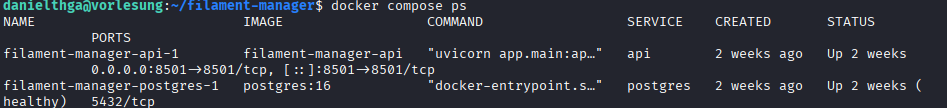
\includegraphics[
    width=\textwidth,
    height=0.42\textheight,
    keepaspectratio
  ]{images/docker-compose-ps.png}
  \caption{Running backend services managed by Docker Compose}
  \label{fig:docker-compose-ps}
\end{figure}

Figure~\ref{fig:docker-compose-ps} shows an example of a correctly running
backend installation. Both the FastAPI and PostgreSQL services are active,
and the API is exposed through the configured host port.

\subsection{Verify the API}

The application uses host port \texttt{8501}.

Test the root endpoint:

\begin{lstlisting}
curl http://localhost:8501/
\end{lstlisting}

Expected response:

\begin{lstlisting}
{"status":"ok","application":"Filament Manager API"}
\end{lstlisting}

Test the health endpoint:

\begin{lstlisting}
curl http://localhost:8501/health
\end{lstlisting}

FastAPI automatically provides interactive API documentation at:

\begin{lstlisting}
http://localhost:8501/docs
\end{lstlisting}

For a remote backend, replace \texttt{localhost} with the hostname or IP
address of the backend server.

% ============================================================
\section{Docker Compose operation}
% ============================================================

Docker Compose is responsible for starting and connecting both backend
services.

The PostgreSQL service provides persistent database storage. The API service
contains the FastAPI application.

The API reaches PostgreSQL using the Compose service name:

\begin{lstlisting}
postgres
\end{lstlisting}

Docker's internal DNS resolves this name inside the Compose network.

Useful commands are:

\begin{lstlisting}
docker compose up -d
docker compose ps
docker compose logs api
docker compose logs postgres
docker compose restart api
docker compose down
\end{lstlisting}

To rebuild the API after changing dependencies or the Dockerfile:

\begin{lstlisting}
docker compose up -d --build api
\end{lstlisting}

\begin{warnbox}
Do not use \texttt{docker compose down -v} on a production installation
unless deletion of the PostgreSQL volume and all stored database data is
explicitly intended.
\end{warnbox}

% ============================================================
\section{Database initialisation}
% ============================================================

The database definition is stored in:

\begin{lstlisting}
database/schema.sql
\end{lstlisting}

Development and test data are stored in:

\begin{lstlisting}
database/seed.sql
\end{lstlisting}

The schema can be loaded manually with:

\begin{lstlisting}
docker compose exec -T postgres \
  psql -U admin -d filament_manager \
  < database/schema.sql
\end{lstlisting}

The seed data can be loaded with:

\begin{lstlisting}
docker compose exec -T postgres \
  psql -U admin -d filament_manager \
  < database/seed.sql
\end{lstlisting}

\subsection{Database inspection}

Open an interactive PostgreSQL shell:

\begin{lstlisting}
docker compose exec postgres \
  psql -U admin -d filament_manager
\end{lstlisting}

List the tables:

\begin{lstlisting}
\dt
\end{lstlisting}

Inspect a table:

\begin{lstlisting}
\d filament_roll
\end{lstlisting}

Exit PostgreSQL:

\begin{lstlisting}
\q
\end{lstlisting}

% ============================================================
\section{Backend source code}
% ============================================================

\subsection{Main API}

The FastAPI routes and main business logic are implemented in:

\begin{lstlisting}
api/app/main.py
\end{lstlisting}

The application implements endpoints for:

\begin{itemize}
  \item filament rolls,
  \item filament types,
  \item stock aggregation,
  \item print models,
  \item print jobs,
  \item filament roll suggestions.
\end{itemize}

\subsection{Pydantic schemas}

Request validation is defined in:

\begin{lstlisting}
api/app/schemas.py
\end{lstlisting}

Pydantic validates incoming JSON before the data reaches the database logic.

Invalid values such as negative filament quantities are therefore rejected
with an HTTP 4xx response.

\subsection{Database access}

Database connection handling is implemented in:

\begin{lstlisting}
api/app/database.py
\end{lstlisting}

The backend uses \texttt{psycopg2} to access PostgreSQL.

\subsection{Authentication}

API-key validation is implemented in:

\begin{lstlisting}
api/app/auth.py
\end{lstlisting}

Write operations require:

\begin{lstlisting}
X-API-Key: <configured-api-key>
\end{lstlisting}

Read endpoints do not require the key.

% ============================================================
\section{REST API}
% ============================================================

FastAPI automatically generates interactive OpenAPI documentation for the
implemented REST interface. This provides developers with an overview of the
available routes and allows requests to be inspected and tested directly from
a web browser.

\begin{figure}[htbp]
  \centering
  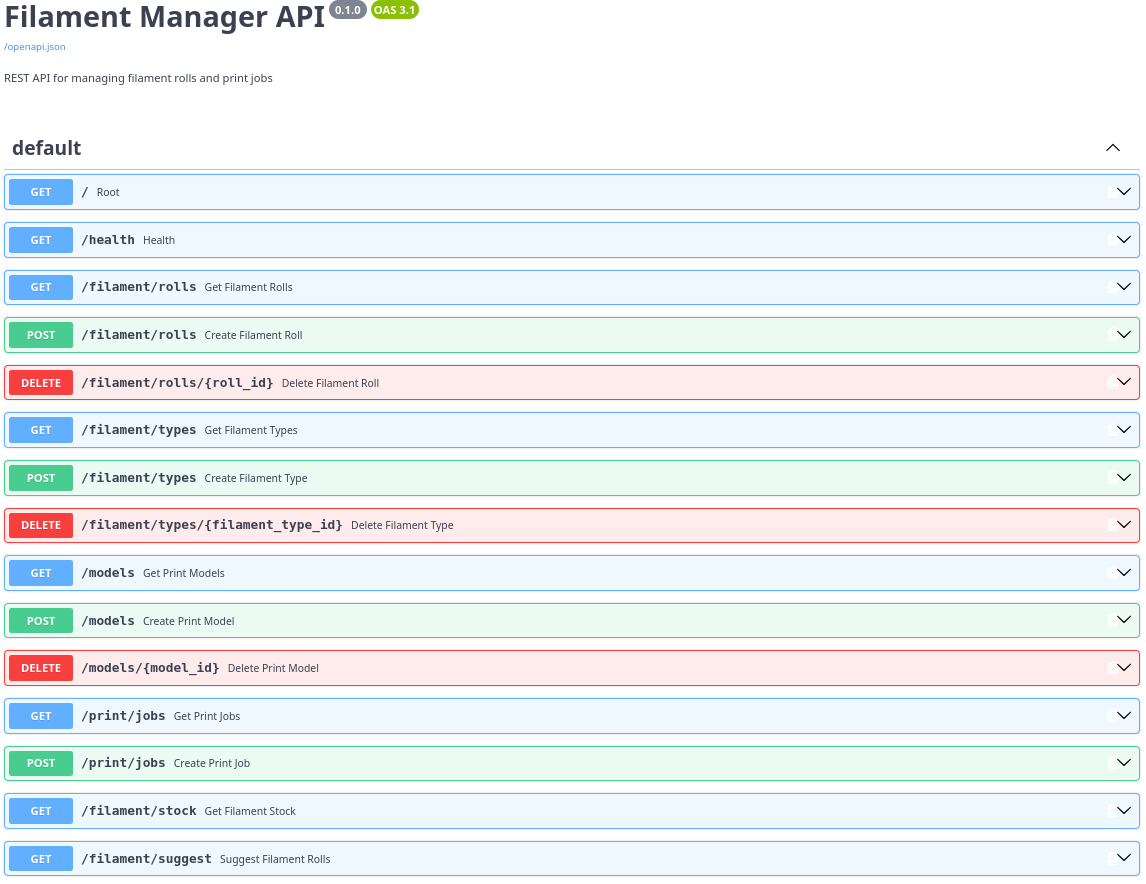
\includegraphics[
    width=\textwidth,
    height=0.58\textheight,
    keepaspectratio
  ]{images/fastapi-swagger.png}
  \caption{Interactive FastAPI documentation of the Filament Manager API}
  \label{fig:fastapi-swagger}
\end{figure}

The Swagger interface shown in Figure~\ref{fig:fastapi-swagger} is available
through the \texttt{/docs} endpoint of the running backend. It is particularly
useful during development for inspecting request parameters, response schemas
and HTTP methods.

The following table summarises the central API routes.

\begin{tabularx}{\linewidth}{@{}p{1.7cm}p{5cm}X@{}}
\toprule
\textbf{Method} & \textbf{Path} & \textbf{Purpose} \\
\midrule

GET
& \texttt{/filament/rolls}
& Returns all filament rolls including joined type information. \\

POST
& \texttt{/filament/rolls}
& Creates a filament roll. Requires X-API-Key. \\

DELETE
& \texttt{/filament/rolls/\{id\}}
& Deletes an unused filament roll. Requires X-API-Key. \\

GET
& \texttt{/filament/types}
& Returns all filament types. \\

POST
& \texttt{/filament/types}
& Creates a filament type. Requires X-API-Key. \\

DELETE
& \texttt{/filament/types/\{id\}}
& Deletes an unused filament type. Requires X-API-Key. \\

GET
& \texttt{/filament/stock}
& Returns aggregated stock information. \\

GET
& \texttt{/filament/suggest}
& Selects suitable filament roll allocations. \\

GET
& \texttt{/models}
& Returns all print models. \\

POST
& \texttt{/models}
& Creates a print model. Requires X-API-Key. \\

DELETE
& \texttt{/models/\{id\}}
& Deletes an unused print model. Requires X-API-Key. \\

GET
& \texttt{/print/jobs}
& Returns print history using several JOIN operations. \\

POST
& \texttt{/print/jobs}
& Creates a print job and updates filament inventory.
  Requires X-API-Key. \\

\bottomrule
\end{tabularx}

% ============================================================
\section{Filament allocation business rule}
% ============================================================

One of the central features of the application is the automatic selection of
filament rolls.

The backend receives:

\begin{itemize}
  \item a filament type,
  \item the amount of filament required for the print.
\end{itemize}

Available rolls of the requested filament type are ordered by their remaining
weight.

\subsection{Single-roll selection}

If one roll contains enough filament, the smallest sufficient roll is used.

For example, assume the available rolls contain:

\begin{lstlisting}
180 g
620 g
950 g
\end{lstlisting}

If a print requires \texttt{500 g}, the \texttt{620 g} roll is selected.

The larger \texttt{950 g} roll is preserved.

\subsection{Multiple-roll allocation}

If no single roll contains enough filament, but the sum of all matching rolls
is sufficient, the backend uses multiple rolls.

For a \texttt{1000 g} print, an example allocation could be:

\begin{lstlisting}
Roll 1: 180 g
Roll 2: 620 g
Roll 7: 200 g
\end{lstlisting}

This is recorded through the N:M relationship between
\texttt{print\_job} and \texttt{filament\_roll}.

\subsection{Insufficient filament}

If the combined amount is too small, the API returns:

\begin{lstlisting}
HTTP 409 Conflict
\end{lstlisting}

No print job is created and no filament quantity is changed.

\subsection{Transactions}

Creating a print job consists of several database changes:

\begin{enumerate}
  \item create the print job,
  \item create one or more \texttt{print\_job\_roll} records,
  \item reduce the remaining weight of every selected roll.
\end{enumerate}

These changes are executed within one transaction.

This guarantees that either all modifications are committed or none of them
are applied.

% ============================================================
\section{Backend testing}
% ============================================================

Automated backend tests are located in:

\begin{lstlisting}
api/tests/test_api.py
\end{lstlisting}

A separate PostgreSQL database is used for testing:

\begin{lstlisting}
filament_manager_test
\end{lstlisting}

This prevents automated tests from modifying development or production data.

\subsection{Create the test database}

If it does not yet exist:

\begin{lstlisting}
docker compose exec postgres \
  psql -U admin -d postgres \
  -c "CREATE DATABASE filament_manager_test;"
\end{lstlisting}

Load test data:

\begin{lstlisting}
docker compose exec -T postgres \
  psql -U admin -d filament_manager_test \
  < database/seed.sql
\end{lstlisting}

\subsection{Run the tests}

Execute:

\begin{lstlisting}
docker compose exec \
  -e POSTGRES_DB=filament_manager_test \
  api pytest -v -p no:cacheprovider tests
\end{lstlisting}

The implemented test suite verifies:

\begin{itemize}
  \item root endpoint availability,
  \item filament roll retrieval,
  \item stock aggregation,
  \item rejection of write requests without a valid API key,
  \item validation of invalid model data,
  \item selection of the smallest sufficient roll,
  \item handling of insufficient filament.
\end{itemize}

All automated tests should pass before a new backend version is released.

\begin{figure}[htbp]
  \centering
  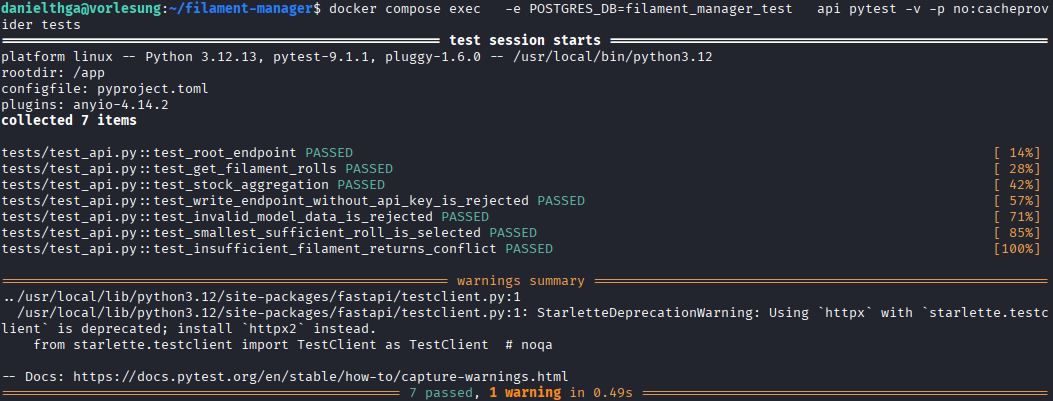
\includegraphics[
    width=\textwidth,
    height=0.50\textheight,
    keepaspectratio
  ]{images/pytest-results.png}
  \caption{Successful execution of the automated backend test suite}
  \label{fig:pytest-results}
\end{figure}

Figure~\ref{fig:pytest-results} shows the expected result of the automated
test suite. All seven implemented tests complete successfully. Developers
should reproduce this result after relevant backend modifications before
committing or releasing a new version.

% ============================================================
\section{Frontend setup on a new development system}
% ============================================================

The frontend is developed separately from the backend.

\subsection{Requirements}

The development system requires:

\begin{itemize}
  \item Linux,
  \item Python 3.11 or newer,
  \item Tkinter,
  \item Git,
  \item uv,
  \item network access to the backend.
\end{itemize}

On Debian-based systems install Tkinter with:

\begin{lstlisting}
sudo apt update
sudo apt install python3-tk
\end{lstlisting}

Check Python:

\begin{lstlisting}
python3 --version
\end{lstlisting}

Check uv:

\begin{lstlisting}
uv --version
\end{lstlisting}

\subsection{Clone the frontend repository}

\begin{lstlisting}
git clone <FRONTEND-REPOSITORY-URL>
cd filament-manager-frontend
\end{lstlisting}

\subsection{Install dependencies}

The project dependencies are defined in:

\begin{lstlisting}
pyproject.toml
\end{lstlisting}

Exact resolved versions are stored in:

\begin{lstlisting}
uv.lock
\end{lstlisting}

Create or synchronise the environment:

\begin{lstlisting}
uv sync
\end{lstlisting}

\begin{infobox}
The \texttt{uv.lock} file is intentionally committed to Git. It ensures that
developers can reproduce the same dependency environment on different
machines.
\end{infobox}

\subsection{Start the frontend}

Start the application directly from the source repository:

\begin{lstlisting}
uv run python -m filament_manager_frontend
\end{lstlisting}

Alternatively use the configured console entry point:

\begin{lstlisting}
uv run filament-manager-frontend
\end{lstlisting}

The application first displays the connection dialog.

For a local backend use:

\begin{lstlisting}
http://localhost:8501
\end{lstlisting}

For a remote backend use:

\begin{lstlisting}
http://<backend-server>:8501
\end{lstlisting}

The X-API-Key configured in the backend must also be entered in the
connection dialog.

% ============================================================
\section{Frontend architecture}
% ============================================================

The frontend separates HTTP communication and graphical user-interface code.

Figure~\ref{fig:frontend-main-window} shows the main window of the completed
desktop application after a successful connection to the backend.

\begin{figure}[htbp]
  \centering
  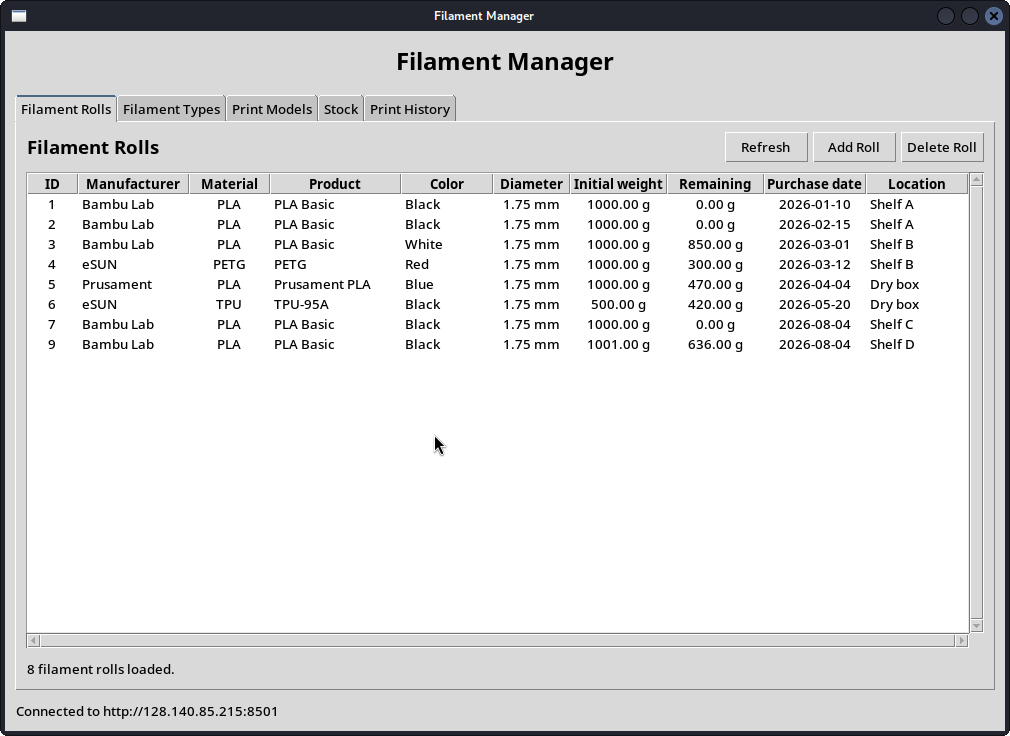
\includegraphics[
    width=\textwidth,
    height=0.55\textheight,
    keepaspectratio
  ]{images/frontend-main-window.png}
  \caption{Main window of the Filament Manager desktop frontend}
  \label{fig:frontend-main-window}
\end{figure}

The graphical interface is organised into separate functional areas. The
individual tabs retrieve their data through the shared API client rather than
accessing PostgreSQL directly.

\subsection{API client}

HTTP communication is implemented in:

\begin{lstlisting}
src/filament_manager_frontend/api.py
\end{lstlisting}

The \texttt{ApiClient} class provides methods for the REST operations.

The GUI itself does not need to construct HTTP requests manually.

\subsection{Application entry point}

The application starts through:

\begin{lstlisting}
src/filament_manager_frontend/__main__.py
\end{lstlisting}

This module:

\begin{enumerate}
  \item creates the Tkinter root window,
  \item opens the connection dialog,
  \item creates the API client,
  \item verifies the connection,
  \item opens the main window.
\end{enumerate}

\subsection{Main window}

The central user interface is located in:

\begin{lstlisting}
src/filament_manager_frontend/ui.py
\end{lstlisting}

It creates the notebook containing the individual application tabs.

\subsection{Tabs}

The following tabs are implemented:

\begin{itemize}
  \item \textbf{Filament Rolls},
  \item \textbf{Filament Types},
  \item \textbf{Print Models},
  \item \textbf{Stock},
  \item \textbf{Print History}.
\end{itemize}

Each tab is implemented in a separate module below:

\begin{lstlisting}
src/filament_manager_frontend/tabs/
\end{lstlisting}

\subsection{Dialogs}

User input is handled by dedicated dialog classes:

\begin{itemize}
  \item Add Filament Roll,
  \item Add Filament Type,
  \item Add Print Model,
  \item Start Print.
\end{itemize}

They are located below:

\begin{lstlisting}
src/filament_manager_frontend/dialogs/
\end{lstlisting}

This separation keeps the individual GUI modules manageable.

% ============================================================
\section{Building the Python frontend package}
% ============================================================

The frontend uses a standard Python package definition in:

\begin{lstlisting}
pyproject.toml
\end{lstlisting}

Build the package with:

\begin{lstlisting}
uv build
\end{lstlisting}

The build creates:

\begin{lstlisting}
dist/filament_manager_frontend-0.1.0-py3-none-any.whl
dist/filament_manager_frontend-0.1.0.tar.gz
\end{lstlisting}

\subsection{Clean package test}

Create an independent test environment:

\begin{lstlisting}
uv venv /tmp/filament-manager-test
\end{lstlisting}

Install the wheel:

\begin{lstlisting}
uv pip install \
  --python /tmp/filament-manager-test/bin/python \
  dist/*.whl
\end{lstlisting}

Verify the installed packages:

\begin{lstlisting}
uv pip list \
  --python /tmp/filament-manager-test/bin/python
\end{lstlisting}

Start the installed application:

\begin{lstlisting}
/tmp/filament-manager-test/bin/filament-manager-frontend
\end{lstlisting}

The frontend must start without depending on the source repository.

% ============================================================
\section{Debian package}
% ============================================================

For Linux deployment, the frontend is additionally packaged as a Debian
package.

The package contains:

\begin{itemize}
  \item the Python wheel,
  \item Debian package metadata,
  \item an installation script,
  \item an executable launcher.
\end{itemize}

\subsection{Build the package}

From the frontend repository:

\begin{lstlisting}
dpkg-deb --build --root-owner-group \
  packaging/filament-manager-frontend_0.1.0_all
\end{lstlisting}

The resulting package is:

\begin{lstlisting}
packaging/filament-manager-frontend_0.1.0_all.deb
\end{lstlisting}

\subsection{Install the package}

Install it with:

\begin{lstlisting}
sudo apt install \
  ./packaging/filament-manager-frontend_0.1.0_all.deb
\end{lstlisting}

After installation the application can be launched globally:

\begin{lstlisting}
filament-manager-frontend
\end{lstlisting}

Verify the installation:

\begin{lstlisting}
dpkg -l | grep filament-manager
which filament-manager-frontend
\end{lstlisting}

The expected launcher path is:

\begin{lstlisting}
/usr/bin/filament-manager-frontend
\end{lstlisting}

Remove the application with:

\begin{lstlisting}
sudo apt remove filament-manager-frontend
\end{lstlisting}

% ============================================================
\section{Development workflow}
% ============================================================

Before starting development, update the local repository:

\begin{lstlisting}
git pull
git status
\end{lstlisting}

After implementing a change:

\begin{enumerate}
  \item inspect the changed files,
  \item test the application,
  \item review the Git diff,
  \item stage the relevant files,
  \item commit the change,
  \item push it to the remote repository.
\end{enumerate}

Example:

\begin{lstlisting}
git status
git diff
git add <changed-files>
git commit -m "feat: describe the change"
git push
\end{lstlisting}

Common commit prefixes used in the project are:

\begin{tabularx}{\linewidth}{@{}p{2.5cm}X@{}}
\toprule
\textbf{Prefix} & \textbf{Purpose} \\
\midrule

\texttt{feat}
  & New functionality. \\

\texttt{fix}
  & Bug fix. \\

\texttt{test}
  & Automated or manual test changes. \\

\texttt{docs}
  & Documentation changes. \\

\texttt{build}
  & Build-system or package changes. \\

\texttt{chore}
  & Maintenance work. \\

\bottomrule
\end{tabularx}

% ============================================================
\section{Troubleshooting}
% ============================================================

\subsection{Backend does not start}

Check the current container state:

\begin{lstlisting}
docker compose ps
\end{lstlisting}

Inspect API logs:

\begin{lstlisting}
docker compose logs api
\end{lstlisting}

Inspect PostgreSQL logs:

\begin{lstlisting}
docker compose logs postgres
\end{lstlisting}

\subsection{Database connection fails}

Ensure that PostgreSQL reports a healthy state:

\begin{lstlisting}
docker compose ps
\end{lstlisting}

Inside the Docker Compose environment, the API must use:

\begin{lstlisting}
postgres
\end{lstlisting}

as the database hostname, not \texttt{localhost}.

\subsection{API returns HTTP 403}

Protected write endpoints require the correct X-API-Key.

Check that the value entered in the frontend matches the value configured in
the backend \texttt{.env} file.

\subsection{Frontend cannot reach the backend}

Test the backend directly from the frontend computer:

\begin{lstlisting}
curl http://<backend-address>:8501/health
\end{lstlisting}

If this request fails, investigate:

\begin{itemize}
  \item server address,
  \item Docker container status,
  \item port mapping,
  \item firewall settings,
  \item network connectivity.
\end{itemize}

\subsection{Python import error}

Synchronise the environment:

\begin{lstlisting}
uv sync
\end{lstlisting}

Verify the package import:

\begin{lstlisting}
uv run python -c \
  "import filament_manager_frontend; \
   print(filament_manager_frontend.__file__)"
\end{lstlisting}

% ============================================================
\section{Security considerations}
% ============================================================

The following rules should be followed during development and deployment:

\begin{itemize}
  \item Never commit the real \texttt{.env} file.
  \item Never commit database passwords or API keys.
  \item Keep only \texttt{.env.example} in Git.
  \item Use a separate database for automated tests.
  \item Do not give the desktop frontend direct database access.
  \item Do not expose the PostgreSQL port unnecessarily.
  \item Validate modifications through the REST API.
\end{itemize}

The API key is entered by the frontend user when the application starts and
is kept only for the current application session.

% ============================================================
\section{Extending the application}
% ============================================================

A new feature should follow the existing separation between database,
backend and frontend.

For a database-backed feature:

\begin{enumerate}
  \item Modify \texttt{database/schema.sql} if required.
  \item Update \texttt{database/seed.sql} if new development data is needed.
  \item Add or modify Pydantic schemas in
        \texttt{api/app/schemas.py}.
  \item Add the REST operation in \texttt{api/app/main.py}.
  \item Add automated backend tests.
  \item Add the corresponding method to the frontend
        \texttt{ApiClient}.
  \item Add or modify the required Tkinter tab or dialog.
  \item Test the complete workflow.
  \item Commit and push the source code.
\end{enumerate}

Operations involving several dependent database modifications should use a
transaction.

% ============================================================
\section{Release checklist}
% ============================================================

Before creating a new release:

\begin{itemize}[label=$\square$]
  \item Pull the latest source code.
  \item Verify that no secrets are staged in Git.
  \item Build the backend containers.
  \item Verify the PostgreSQL health check.
  \item Verify the API health endpoint.
  \item Run all automated backend tests.
  \item Start the frontend using \texttt{uv run}.
  \item Test the frontend/backend connection.
  \item Build the Python wheel.
  \item Test the wheel in a clean virtual environment.
  \item Build the Debian package.
  \item Install and start the Debian package.
  \item Commit all required source changes.
  \item Push all repositories.
\end{itemize}

% ============================================================
\section{Conclusion}
% ============================================================

The Filament Manager uses a clear separation between the PostgreSQL database,
FastAPI backend and Tkinter desktop application.

Docker Compose provides a reproducible runtime environment for the backend,
while \texttt{uv} provides reproducible dependency management for the
frontend. The REST API forms the only communication interface between both
parts of the system.

Automated backend tests, Git version control and separate packaging steps make
the system reproducible and maintainable on other development systems.

The architecture allows individual layers to be modified without requiring a
complete redesign of the application.

\end{document}
